%
%
%
\chapter{Spin-Fermion-Model}
\label{ch: spin fermion model}
%
%
%
In the following chapter the spin-fermion-model for a metal exhibiting a antiferromagnetic quantum phase transition is introduced as presented in \cite{Abanov&Chubukov&Schmalian}.
Beside fermionic particle-hole-exitetaions in the vicinity of the quantum critical point bosonic spin fluctuations arise in this low energy theory, which enable a attractive interaction between electrons.
This chapter isn't displayed a detailed mathematical or microscopic derivation of the spin-fermion-model, but rather it is based on a qualitative description to justified its form.
In particular, we focus one's attention on the arising spin fluctuations, agrue them carry large momenta and introduced the damped spin density propagator and their perodicity.
Further we present the basic concepts of hot-spot theory, which are points on the Fermi surface in 2D cutting by the magnetic Brillouin zone.
Besides we review excplicitly the conservation of momentum and non-conservation of current for the observing Hamiltonian.
For breaking translation symmetry umklapp scattering is introduced and we prove that this is unconserving momentum.
%
%
\section{Spin-Fermion-Model}
\label{sec:spin-fermion-model}
%
%
%
\begin{figure}[t]
	\centering
	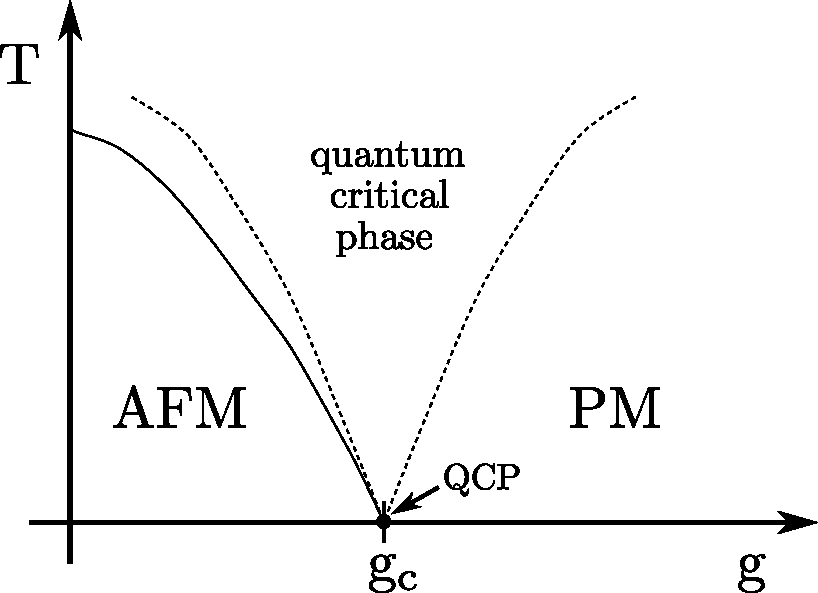
\includegraphics[width=0.7\textwidth]{phase_diagram.pdf}
	\caption{
This figure shows a shematic and simplified phase diagram for metals transition from a paramagnetic (PM) into an antiferrmagnetic (AFM) phase depending on a tunung parameter g.
The phase line of the AFM phase ends decreasing temperature down to $T = 0$ in a quantum critical point (QCP) at $\mt{g} = \mt{g}_{\mt{c}}$.
At this point the phase transition is only caused by quantum fluctuations.
At $T > 0$ thermal fluctuactions more and more dominates the phase transition.
Nevertheless quantum fluctuations influences the physical behaviour in a lagre regime, labeled as quantum critical phase.
	}
	\label{fig:phase diagram}
\end{figure}



\begin{itemize}
	\item explain the quantum critical point theory
	\item introduced the spin fermion model in detail used by Sachdev and me
	\item difference two other spin fermion models and why these changes are important
	\item show that the momentum is conserved and the current dosen't
	\item introduced the pertubation Hamiltonian which included umklapp scattering
	\item show that the current doesn't change and the momentum isn't anymore conserved
\end{itemize}